\section{Basics: Functional Programming in Coq}

%%%%%%%%%%%%%%%%%%%%%%%%%%%%%%%%%%%%%
	\subsection{Introduction}
%%%%%%%%%%%%%%%%%%%%%%%%%%%%%%%%%%%%

	In this chapter we are going to introduce the most essential elements of Coq's functional programming language called {\itshape Gallina}. 
	Moreover, {\itshape tactics} which can be applied to prove properties of Coq programs are introduced (subsection \ref{subsec:proof-techniques} and \ref{subsec:proofByCaseAnalysis}).
	
%%%%%%%%%%%%%%%%%%%%%%%%%%%%%%%%%%%%%
	\subsection{Data and Functions}
	\label{subSec:DataAndFuctions}
%%%%%%%%%%%%%%%%%%%%%%%%%%%%%%%%%%%%%
	
	 \paragraph{Enumerated Type}
	 
	 
	  The built-in features set in Coq is extremely small. In particular, Coq is a powerful mechanism for defining data types from scratch.
	  Current Coq distributions come preloaded with an extensive standard library containing Boolean, numbers, data structures like lists and hash tables.\\
	  
	  In this course we are going to explicitly recapitulate the used definitions. 
	  It is started by a rather simple example of a self-defined type.  
	   
	  
	  \begin{example}
	  We are defining a type called \lstinline!day!.~\\\vspace{-10mm}
	  {\normalfont \begin{lstlisting} [caption={\lstinline!day!}] 
	    Inductive day: Type :=
		  | monday
		  | tuesday
		  | wednesday
		  | thursday
		  | friday
		  | saturday
		  | sunday.
	  \end{lstlisting}}
	  The type members are called \lstinline!monday!, \lstinline!tuesday! , \lstinline!wednesday! \ldots{} and \lstinline!sunday!.\\
	  We are defining a function operating on \lstinline!day!: 
	  {\normalfont \begin{lstlisting}[caption = {\lstinline! next_weekday!}]
	  Definition next_weekday(d:day) day:=
	    match d with 
		  | monday => tuesday
		  | tuesday => wednesday
		  | wednesday => thursday
		  | thursday => friday
		  | friday => monday
		  | saturday => monday
		  | sunday => monday
	    end.  
	  \end{lstlisting}}
	  \end{example}
	  Coq is able of {\itshape type  interference}, whenever the type is not defined explicitly.
	  But for readability, we are including types in the following.
	 Note that the keyword for function is \lstinline!Definition! and the type if called \lstinline!Inductive!. 
	 We are calling the data-type \lstinline!day! an inductively defined data-type. 	 
	 \\   
	  
	  For testing the above definition and function we have three possibilities in Coq:
	     
	   \begin{enumerate}
	   \item Compute a compound expression including the function:\\ 		
	 		 \lstinline! compute (next_weekday friday).! Coq output: \lstinline!\nbsp	 = monday : day ! or \\
	 		 \lstinline! compute (next_weekday (next_weekday saturday)).! Coq output: \lstinline! = tuesday : day !\\ 	      
	   \item Record an expected behaviour as a Coq-\lstinline!Example! and verify the assertion:\\ 
	         {\itshape The second weekday after Saturday is Tuesday.}     
			   \begin{lstlisting}
			   		Example. test_next_weekday: (next_weekday (next_weeekday(saturday)) = tuesday 
			   		Proof. simpl. reflexivity. Qed.
			   \end{lstlisting}
	   			The details of the implementation are not important right now. 
	   			We are going to come back to them later.
	   
	   \item \label{CoqAsCodeGen} Moreover, Coq can be asked to \lstinline!extract! a program from our \lstinline! Definition! in a programming language which is more conventional, being equipped with a high performance compiler.
	    In particular this is one of the main uses of Coq. 
	    It provides a method to transfer proved-correct algorithms in Gallina to efficient machine code (see section \ref{sec:coqAsACodeGenerator}).
	    (Assuming the correctness of the corresponding high performance compiler e.g. the Ocaml, Haskell or Scheme compiler.) 			
	   \end{enumerate}   
	
%%%%%%%%%%%%%%%%%%%%%%%%%%%%%%%%%%%%%
	\subsection{Boolean}
%%%%%%%%%%%%%%%%%%%%%%%%%%%%%%%%%%%%%
	
	    Of course, Coq provides an default implementation of Boolean.
	    (See the \newline \href{https://www.cs.princeton.edu/courses/archive/fall07/cos595/stdlib/html/Coq.Init.Datatypes.html}{Coq.Init.Datatypes \allowbreak in the Coq-Library documentation}).  
	    In the following we are going to be consistent with the Coq library documentation according to the standard library.
	    We are going to introduce coinciding self-defined data types whenever possible.\\
	    Boolean can be defined as follows:
	    
	    \label{Def:booleans}
	    \begin{lstlisting}[caption= \lstinline!bool!]    
	    Inductive bool: Type :=
	      | true
	      | false.
	    \end{lstlisting}
	     A function with multiple input arguments is implemented by
	    \begin{lstlisting}[caption = \lstinline!orb!, label = lst:orb]
	    Definition orb (b1: bool) (b2: bool) : bool :=
	    match b1 with
		  | true -> true
		  | false -> b2
	    end.
	    \end{lstlisting}    
	    The functions \lstinline!negb! and \lstinline!andb!, corresponding to the Boolean functions {\emph negation} and {\emph and}, are implemented in a similar manner.\\   
	    And a new symbolic notations is implemented as follows:
	    \begin{lstlisting}[caption= introducing a new notation]
	    Notation "x && y" := (andb x y).
	    Notation "x||y" := (orb x y).
	    \end{lstlisting}
	    
%%%%%%%%%%%%%%%%%%%%%%%%%%%%%%%%%%%%%	     
	\subsection{Some Notation}
%%%%%%%%%%%%%%%%%%%%%%%%%%%%%%%%%%%%%	
	    As in the Coq doc documentation tool the following notation convention is introduced:
	     
	    \begin{enumerate}
	     \item In \texttt{.v-files} comments are annotated by \lstinline!(* some comment *)!. 
	     \item Within these comments Coq-code is denoted by \lstinline![example].! 
	     \item And we write \lstinline! Admitted.! at the end of an incomplete proof.    
	     \end{enumerate}
	     
%%%%%%%%%%%%%%%%%%%%%%%%%%%%%%%%%%%%%	     
	\subsection{Types}
%%%%%%%%%%%%%%%%%%%%%%%%%%%%%%%%%%%%%
	     Every expression in Coq has a type, which can be revealed by \lstinline!check!. 
	     \begin{enumerate}
	      \item  \lstinline* Check true.* gives the type of the expression \lstinline! boolean!.
	      \item \lstinline! Check negb.! returns \lstinline! bool -> bool! . (Read as  ``bool arrow bool'').
	              It is the function's input data type and the output data type, given input data of that type.
	       \item \lstinline! andb! returns \lstinline!bool->bool->bool!. This function produces an output of type \lstinline! bool! given two inputs of type \lstinline! bool!.
	     \end{enumerate}

%%%%%%%%%%%%%%%%%%%%%%%%%%%%%%%%%%%%%	   
	\subsection{New Types from Old}
%%%%%%%%%%%%%%%%%%%%%%%%%%%%%%%%%%%%%
	          
		 Note that so far the data-types we have seen were enumerated types.
		 Let's define a data type \lstinline!rgb! and a data type \lstinline!primary!, whose constructor takes this type as an argument.
		 
	    \begin{minipage}[t]{0.45\textwidth}
		\begin{lstlisting}[caption = \lstinline!rgb!, label = lst:rgb]
		 Inductive rgb: Type:=
		  | red     (* These are the *)
		  | green   (* expressions in *)
		  | blue.   (* the set [rgb]. *)
		 \end{lstlisting}
		 The constructors of the type \lstinline!rgb! are \lstinline!red, green! and \lstinline!blue!. 
		 \end{minipage}
		 \hfill	 
		 \begin{minipage}[t]{0.45\textwidth}
		 \begin{lstlisting}[caption = \lstinline!color!, label = lst:color ]
		 Inductive color: Type := 
		  | black  (* An expression in the set color *)
		  | white  (* An expression in the set color *)
		  | primary (p:rgb). (* If [p] is in the set [rgb], then the constructor [primary] applied to the argument [p] is an expression in the set color.*) 
		 \end{lstlisting}
		 The constructors of the type \lstinline!color! are \lstinline!black, white! and \lstinline!primary!.\\
		 %The expressions in the set color are \lstinline!black, white! and \lstinline!primary! if primary is fomed as above.
		 \end{minipage}	 	 
		 
		 Note that expressions formed as in listing \lstinline!rgb! and \lstinline!color! (see  listing \ref{lst:rgb} and  \ref{lst:color}) are the only ones belonging to the sets \lstinline!rgb! and \lstinline!color!.
		 A function on this struct can by defined by patternmatching just as in the previus example (listing \ref{lst:orb}).
		 \begin{lstlisting}[caption = \lstinline!monochrome! , label = lst:monochrome]
		 Definition monochrome (c : color) : bool :=
			  match c with
			  | black => true
			  | white => true
			  | primary q => false
			  end.
		 \end{lstlisting}


		 
%%%%%%%%%%%%%%%%%%%%%%%%%%%%%%%%%%%%%	
	\subsection{Tuples}
%%%%%%%%%%%%%%%%%%%%%%%%%%%%%%%%%%%%%
	
	    A single constructor with multiple parameters can be used to create a type \lstinline!tuple!.
		\begin{example}[A nibble: half a byte]~\\\vspace{-10mm}
	 	 	{\normalfont 
	 	 	    \begin{lstlisting}[caption = \lstinline!bit! and \lstinline!nibbel!]
	 	 		Inductive bit: Type := (* a bit *) 
	 	 		 |B0
	 	 		 |B1.
	 	 		 
	 		    Inductive nibble: Type := (* a nibble *)
	 		   	 |bits( b0 b1 b2 b3: bit).
	 		   			 	
	 		   	Check(bits B1 B0 B1 B0) (* => bits B1 B0 B1 B0 : nibble *)
	 		\end{lstlisting}
	 		Hence, a tuple of four bits is a nibble.\\ 		
	 		Assume we would like to test a nibbel in order to see if all it's bits are 0. 
	 		The nibble is unwrapped by pattern-matching:
	 		\begin{lstlisting}[caption = \lstinline!all_zero!]
	 		Definition all_zero(nb: nibble): bool :=
	 		  match nb with
	 	  	    |(bits B0 B0 B0 B0) -> true
	 		    |(bits _ _ _ _ ) -> false (* This wildcard pattern was included to avoid inventing variable names, which are not going to be used. *) 
	 		  end.
	 		 \end{lstlisting}}
	 	\end{example}
	 	
%%%%%%%%%%%%%%%%%%%%%%%%%%%%%%%%%%%%%	
	\subsection{Modules}
%%%%%%%%%%%%%%%%%%%%%%%%%%%%%%%%%%%%%
	
		Coq provides a {\itshape module system} to aid organizing large developments (like Packages in Java (see \cite[Section 3.6.5]{U}).
		In this course most of it is not going to be needed. Namespaces use the $.$-notation as in C++ Data structures (see \cite{CppDotComDS}).
	
		\begin{lstlisting}[caption = \lstinline!Module!]
		Module X 
		...
		... foo... (* a definition declared as foo *)
		...
		End X
		
		X.foo (* Referes to foo, which is definded in the module X. *)
		\end{lstlisting}
		
%%%%%%%%%%%%%%%%%%%%%%%%%%%%%%%%%%%%%	
	\subsection{Numbers}
%%%%%%%%%%%%%%%%%%%%%%%%%%%%%%%%%%%%%
	
	  Note that on the one hand the types day, bool, bits and tuples have a finite set of values, while on the other hand the set of natural numbers $\mathbb{N}$ is an infinite set.\\ 
	  Hence, we have to construct $\mathbb{N}$ using a data type with a finite number of constructors. 
	  Recall, that many representations of $\mathbb{N}$ exist (e.g. hexadecimal with base 16, octa with base 8, binary with base 2).
	  The most familiar might be the decimal representation.\\
	  However, each representation of $\mathbb{N}$ can be useful under different circumstances. 
	  The binary representation is valuable in computer hardware, because it presents a simple circuitry.
	  Here simple proofs are aimed using the unary (base 1) representation.
	  
	  \begin{lstlisting}[caption={\lstinline!nat!}, label=lst:DefNat]
	  Module NatPlayground
	  
	  Inductive nat: Type :=
	    | 0
	    | S (n:nat).
	  \end{lstlisting}  
	  The two constructors of the set \lstinline!nat! are \lstinline!S! and \lstinline!0!. \\
	
	 % One might picture this representation by strokes on a coaster in a beer garden.                                                       
	 One might picture this representation by strokes in the beergarden.  
	 (Actually the definition in listing \ref{lst:DefNat} is an inductive definition as delinated in the Appendix \ref{subsec:InduktiveDefinition}.)	  
	  \begin{itemize}
	  \item The expression \lstinline!0! is in the set \lstinline!nat!.
	  \item The expression \lstinline!0! represents the natural number zero. 
	  \item If \lstinline!n! is an expression belonging to the set \lstinline!nat!, then \lstinline!Sn! represents a natural number $n\in\mathbb{N}\setminus\{ 0\}$.  
	  \end{itemize}	  
	  
	  There is a way of converting this representation refereed to as \lstinline!nat! into it's decimal representation. 
	  This is elaborated in example \ref{ex:ConvertingUnaryToDecimal}.
	  \begin{example}[Converting Unary to Decimal] \label{ex:ConvertingUnaryToDecimal} ~\\%\vspace{mm}
	  \begin{center}  
		  \begin{tabular} {r l}
		  
			  \texttt{unary}				& \texttt{decimal}	\\
			  \texttt{\lstinline!0!} 		&: 0 				\\
			  \texttt{\lstinline! S 0!}  	&: 1				\\
			  \texttt{\lstinline! S ( S 0)!}	&: 2			\\
			  \texttt{\lstinline! S( S ( S 0))!}	&: 3		\\
			    
		  \end{tabular}
		  \end{center}
	  \end{example}
	  Moreover, it is easy to see the following: 
	  \begin{itemize}
	  \item The expression \lstinline!0! belongs to the set \lstinline! nat!.
	  \item If \lstinline!n! is in the set \lstinline! nat!, it follows \lstinline! S n ! is an expression belonging to the set \lstinline! nat!.
	  \item And expressions belongs the set \lstinline!nat! if and only if they are  formed by either of those methods (i.e. \lstinline! 0 ! or  \lstinline! S n!). 
	  \end{itemize}  
	  Note that the same rules apply to the definitions of \lstinline! day!, \lstinline! bool! and \lstinline! color!.
	  These conditions are a precise force of the \lstinline! Inductive! declaration. 
	  Expressions build from other data constructors like \lstinline!true!, \lstinline! false!, \lstinline!andb(S(false( 0 ( 0 S ))))! do not belong to this set.  
	  But on the other hand, \lstinline!0! and \lstinline!S! are arbitrary symbols chosen in the defined representation. 
	  Actually the {\itshape interpretation} of these marks is given by their usage in computing.
	  To realize this functions, which ``pattern match'' a representation of natural numbers, are written.\\
	   
	   \begin{figure}[p]
	   	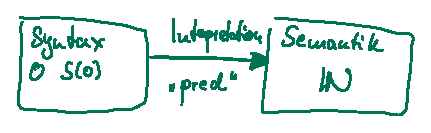
\includegraphics{SemantikSyntax.eps}
	   	\caption{An illustration of function pred. Author: Steffen Reith {\textbf Make a proper figure.}}
	   	\label{fig:SemantikAndSyntaxPred}	     
	   \end{figure}	    

	  We are following the idea:  If n has the form \lstinline!S m! for some \lstinline! m! in the set \lstinline!nat!, then return  \lstinline!m!.
	  \begin{example}[Predecessor Function]%~\\\vspace{-10mm}
	   {\normalfont 
	   Note that although the predecessor of the number zero is not defined, it was declared in listing \ref{lst:pred} for simplicity.    

	   
	   \begin{minipage}[t]{0.45\textwidth}
	   \begin{lstlisting}[caption= \lstinline!pred!, label =lst:pred]
	  	Definition pred (n : nat) : nat := 
	  	  match n with 
	   	    | 0 => 0
	   	    | S m => m
	   	  end. 
	   	  
	    End NatPlayground
	   	 
	    Check pred. 
	    \end{lstlisting}
	    \end{minipage}
	    \hfill
	    \begin{minipage}[t]{0.45\textwidth}
	    \begin{lstlisting}[caption= Coq-output]
	     nat -> nat    
	    \end{lstlisting}
	    \end{minipage}
	   
	    
	  \normalfont }
	  \end{example}
	  
	  Because natural numbers are such a pervasive form of data, Coq always prints out a natural number as decimal by default.
	  (It uses a tiny ``build-in magic'' for paring and printing.)
	 
	  \begin{minipage}[t]{0.50\textwidth}
	  \begin{lstlisting}[caption= \lstinline! minustwo!]
	   Definition minustwo( n: nat) : nat :=
	    match n with
	      | 0 =>  0
	      | S 0 =>  0
	      | S (S m) = > m
	     end.
	     
	   Compute(minustwo(4))
	   \end{lstlisting} 
	   \end{minipage} 
	   \hfill     
	  \begin{minipage}[t]{0.45\textwidth}
	  \begin{lstlisting}[caption = Coq-output] 
	    = 2: nat 
	   \end{lstlisting}
	   \end{minipage}     
	      
	     
	%  So far we have seen the functions \lstinline!S!, \lstinline!pred! and \lstinline!minustwo!.
	  Note that, there is a fundamental difference.
	  The functions \lstinline!pred! and \lstinline!minustwo! apply computational rules. 
	  There are no computational rules about \lstinline!S!.
	  I.e., by the definition of \lstinline!pred!, \lstinline!pred 2! can be simplified to \lstinline!1!. 
	  In the case of \lstinline!S! no such behaviour exists.
	  The definition of \lstinline!S! has no behaviour at all.\\     
	  
	  In order to define more functions over numbers pattern matching used in the definitions of \lstinline!pred! and \lstinline!minustwo! is not sufficient. We are introducing recursion.
	  Recursion in Coq is notated by the keyword \lstinline!Fixpoint!. Note that the previous definitions obviously did not use recursion, because the definitions did not call themseves.
	  
	  \begin{lstlisting}[caption = \lstinline!evenb! and \lstinline!oddb!]
	  Fixpoint evenb (n : nat) : bool :=
	  	match n with
	  	| 0 => true
	  	| S 0 => false
	  	| S (S n') => evenb n'
	  	end.
	  	
	  Definition oddb (n:nat): bool := negb (even bn). (* a simple definition of odd *)
	  	
	  Example test_oddb1: oddb 1 = true
	    	Proof. simpl. reflexivity. Qed.
	  \end{lstlisting}
	   Note that in this proof \lstinline!simpl.! actually has no effect on the goal. 
	   All the work is done by \lstinline!reflexivity!. 
	   We are going to come to back to that later.

	   
%%%%%%%%%%%%%%%%%%%%%%%%%%%%%%%%%%%%%	   
   \subsection{Multi Argument-Function by Recursion}
%%%%%%%%%%%%%%%%%%%%%%%%%%%%%%%%%%%%%
	   
	   \begin{lstlisting}[caption = \lstinline!plus!, label=lst:plus]
	   Module NatPlayground2
	   
	   Fixpoint plus (n : nat) (m : nat): nat :=
	     match n with
	       | 0 => m
	       | S n' => S (plus n' m)
	     end.
	     
	    Compute (plus 3 2).
	   \end{lstlisting}   
	    A notation convention for calling functions with two expressions and matching two expressions with multiple arguments of the same type exist in Coq, too. 
	    See listing \ref{lst:minus_nat}.
	    
	   \begin{lstlisting}[label = lst:minus_nat, caption={ \lstinline!minus! and \lstinline!exp!}]
	    Fixpoint minus (n m: nat): nat :=
	     match n, m with
	       | 0 , _ => 0
	       | S _ , 0 => n
	       | S n', S m' => minus n' m'
	      end.
	      
	     Example test_mult1: (minus 3 2) = 1.
	     
	      
	     End NatPlayground2
	     
	     Fixpoint exp (base power : nat) : nat :=
	       match power with
	         | 0 => S 0
	         | S p => mult base (exp base p)
	       end.
	         
	   \end{lstlisting}
	   
%%%%%%%%%%%%%%%%%%%%%%%%%%%%%%%%%%%%%	        
   \subsection{Introducing Notations}
%%%%%%%%%%%%%%%%%%%%%%%%%%%%%%%%%%%%%	
	
	    For the Coq-parser and Coq-prettifyer's sake we are introducing a new notation:
	    
	    \begin{lstlisting}[caption= operator overloading of \lstinline!+!] 
	     Notation " x + y ":= (plus x y)
	                      (at level 50, left associativity) (* This line is not of interest for our purpose. *)
	                      : nat_scope. (* This line is not of our interest. *)
	                      
	     Check(( 0 + 1 ) + 1).
	    \end{lstlisting}    
	   And in table \ref{tab:operators} some more functions for our purpose are listed.
	   The interested reader is referred to the literature for an exact definition (see table \ref{tab:operators}).  
	   
	   \begin{table}   
	   \begin{tabular}{|c|c|c|c|}
	     \hline 
	 	  notation      & function        & functionality                       & uses           \\  \hline
	 	  x - y         & minus           & subtract two natural numbers        & see listing  \ref{lst:minus_nat} \\  \hline
	      x * y         & mult            & multiply natural numbers            & nested \lstinline!match!es \\  \hline   
	   	  x =? y        & eqb             & test natural numbers                & nested \lstinline!match!es \\  
	  	                &                 & for equality yielding a Boolean     &                \\  \hline
	   	  x <=? y       & leb             & test if a first argument            & nested \lstinline!match!es \\  
	   	                &                 & is less or equal yielding a Boolean &                \\  \hline
	   \end{tabular}
	   \caption{common operators on natural numbers, full implementation can be found in \cite[section: Basics, Functional Programming in Coq: Numbers]{PACGGHSY}}
	   \label{tab:operators}	   
	   \end{table}   
	   
		Note that we when we said that Coq comes with almost nothing built-in, we really mean it.
	    Even equality testing is a user-defined operation.
	    
%%%%%%%%%%%%%%%%%%%%%%%%%%%%%%%%%%%%%	     
	   \subsection{Proof by Simplification}
%%%%%%%%%%%%%%%%%%%%%%%%%%%%%%%%%%%%%
	   
	   Till now we have defined a few data types and functions.
	   Example: We have seen all claims were shown by the same proofs. \lstinline!simple! and \lstinline!reflexivity!. 
	   \lstinline!simpl! simplified equations and \lstinline!reflexivity! checked weather both sides contain identical values.
	   A rule of thumb might say that, \lstinline!simple! can be used to show more simple properties.
	   For example consider the following observation: ``0+n reduces to n, no matter, what n is.''
	   The mathematical precisely formulated statement can be proven by the definition of zero directly.
	   
	   \begin{example}[theorem \lstinline!plus_0_m!] ~\\\vspace{-5mm}
	  	   {\normalfont \begin{lstlisting}[caption=\lstinline!plus_0_n!, label=lst:plus_0_n]
	   		Theorem. plus_0_n: forall n: nat, 0+n = n.
	   		  Proof. intros n. simpl. reflexivity. Qed.
	    	\end{lstlisting}	}	
		\end{example}              
	    \begin{remark}
	    	Reflexivity does not only check weather both sides of an equation contain identical values. 
	    	On top of this it simplifies, which makes it more powerful. 
	    	We have seen \lstinline!simpl! added in examples so we can see the intermediate state.
	    	Therefore, the proof in listing \ref{lst:plus_0_n} can be simplified by omitting \lstinline!simpl!.(See listing \ref{lst:plus0nPrime}.) 
	     \end{remark}	
	
		\begin{lstlisting}[caption={ \lstinline!plus_0_n'!}, label= lst:plus0nPrime]
	    Theorem plus_0_n': forall n: nat, 0 + n = n.
	      Proof: intros n. reflexivity. Qed.	
	    \end{lstlisting}    
	    By looking at the Coq output we can see that \lstinline!reflexivity! somehow tries ``unfolding'' defined terms.\\    
	    Note that \lstinline!example! and \lstinline!theorem! (and \lstinline!Lemma!, \lstinline!Fact!, \lstinline!Remark! and a few other),
	    mean pretty much the same in Coq, while in Mathematics they do not.
	    
	   
%%%%%%%%%%%%%%%%%%%%%%%%%%%%%%%%%%%%%	     
	\subsection{Proof-Techniques}
	\label{subsec:proof-techniques}
%%%%%%%%%%%%%%%%%%%%%%%%%%%%%%%%%%%%%
	    
	    \paragraph{Intros, Simplification and Reflexivity}
	     Whenever a \lstinline!Theorem! starts with \lstinline!forall n!, we might start a proof by the phrase:
	     Assume \lstinline!n! is some natural number. By \lstinline!intros n! we can tell this to Coq.\\
	     A {\itshape tactic} is a command used between \lstinline!Proof! and \lstinline!Qed!, 
	     which guides the process of checking some claim for example the keyword \lstinline!intros!, \lstinline! simpl! and \lstinline!reflexivity! 
	     are tactics.     
	      \begin{remark}{Notation:} 
	     The suffix \lstinline!_l! is pronounced ``on the left'' (see listing \ref{lst:reflexivity}). 
	 	 \begin{lstlisting}[caption = \lstinline!mult_0_l!, label= {lst:reflexivity}]
		 Theorem mult_0_l: forall n: nat, 0 * n = 0.
		   Proof. intros n. reflexivity. Qed.
		 \end{lstlisting}
		 \end{remark} 
	      
	    In order to understand the tactics \lstinline!reflexivity! carefully analyse the Coq-output of listing \ref{lst:reflexivity}.   
	    Let's recall what reflexivity in terms of an equivalence relation means: 
	   \begin{definition}[Equivalence Relation]
	   Assume $x,y\in \mathcal{M}$ an arbitrary set $\mathcal{M}\neq\emptyset$ and $\thicksim\subset A \times A$ an arbitrary relation.
	   Then $\thicksim$ is said to be an equivalence relation if and only if:
	   \begin{enumerate}
	   \item $a\thicksim a$ (reflexivity)
	   \item $a \thicksim b$ if and only if $b \thicksim c$ (symmetry)
	   \item if $a \thicksim b$ and $ b\thicksim c$ then $a \thicksim c$ (transitivity) 
	   \end{enumerate}
	   \end{definition}
	     
	    A more detailed approach of understanding the tactics \lstinline!reflexivity! is elaborated in section \ref{sec:reflexivity}.  
	    However, due to the \href{https://pjreddie.com/coq-tactics/}{Coq tactics index} it is recommended to use reflexivity, if the goal is to prove that something is equals to itself.  
	      
	     \paragraph{Proof by Rewriting} 
	     \label{par:ProofByRewriting}
	     
	     Consider the following example theorem:     
	     %\begin{example}\\
		 \begin{lstlisting}[caption=\lstinline!plus_id_examples!]
		 Theorem plus_id_example: forall n m: nat,
	       n = m -> 
		   n+n = m+m.	 
		 \end{lstlisting}
		 %\end{example}	
		 We would like to show this theorem instead by making a claim about all numbers by looking at the special case when \lstinline!n=m!.
	     \lstinline!->! corresponds to the mathematical implication operator $\implies$. 
	%     The {\itshape tactic} \lstinline! intros!.        
	     Note that the arrow \lstinline!->! tells Coq to rewrite the object of focus from left to right and \lstinline!<-! can be used to rewrite from right to left.\\
	     
	     In order to proof theorem \lstinline!plus_id_example! the theorem's hypothesis is rewritten as shown in listing \ref{lst:plus_id_example_proof}.
	     \begin{lstlisting}[caption = \lstinline!plus_id_example! and it's proof, label= {lst:plus_id_example_proof}]
           Theorem plus_id_example: forall n m: nat,
             n = m ->
             n + n = m + m.
             Proof.
               intros n m.
               intros H.
               rewrite -> H.
               reflexivity.
             Qed.
         \end{lstlisting} 
         For clearity of the semantics this Coq-code's (listing \ref{lst:plus_id_example_proof}) translation to a mathematical proof is listed in table \ref{tab:aMathematicalTranslation}.  
         \begin{table}[h]       
	   	  \begin{center}
	 	    \begin{tabular}{|c|l|l|}	       
	     	\hline
	     	 line no.  & a mathematical translation           & comment  \\  \hline
	     	  1        & Theorem (\verb!plus_id_example!): $\forall n,m \in \mathbb{N}:$ 
	     	                                                  & Declares the statement \\ 
	     	  2         & $n=m$                                & with the name   \\ 
	          3        & $\quad\implies n+n = m+m.$      & \lstinline!plus_id_example! in Coq \\  
		              &      & as \lstinline!subgoal!. \\  \hline
	     	  4        & Proof:                              & Moves the last proven \\   
	     	      	   &                                     & \lstinline!subgoal! into Coq's focus.  \\     \hline
	     	      	                      
	          5         & Assume $n,m \in \mathbb{N}.$        & Moves the universally     \\
	                    &                                     & quantified  variables \lstinline!n!      \\   
	                    &                                     & and \lstinline!m! into the focus.\\     \hline  
	          6         & $H(n,m) :=(n=m).$                 & Moves the hypothesis \lstinline!H! \\ 
	    	                &                                     & of the \lstinline!subgoal! into the    \\   
	    	                &                                     & focus of Coq.\\ \hline 
	          7         & $H(n,m)\implies $                   & Substitutes by H from \\  
	     	            & $\implies( n+n = m+m \Leftrightarrow\ m+m = m+m).$
	     	                    	                              & left to right in the \lstinline!subgoal!.\\
                        &     	                              & Simplifies if possible. \\ \hline
	     	  8         & trivial.                             & We obtained a trivial                 \\ 
	     	            &                                      &  statement. \\ \hline
	    	      9        & $\qed.$                               &  Quod era demonstrandum.  \\  \hline
	    	   	 \end{tabular}
	    	   	   \caption{\lstinline!plus_id_example!'s mathematical translation}
	    	   	   \label{tab:aMathematicalTranslation}  
	         \end{center}          
          \end{table}  
       N	ote that the syntax and semantics of the Coq-code in listing \ref{lst:plus_id_example_proof} can be easily understood by a reader who is familiar with the notation of predicate logic as in \ref{BasisLogik}. 
       The function of the tactics \lstinline!reflexivity! is also similar to the principle of reflexivity in predicate logic (see:  Need a predicate logic reference!). 
       Therefore a one-to-one translation of this listing into predicate logic can be found in appendix \ref{app:AdditionalMaterials} \ref{subsec:CoqAndPredicateLogic}.  \\      
         
	   \lstinline!rewrite! can also be used with a previously proven theorem instead of a hypothesis of context.
	   If the statement of the previously proven theorem involves prequantified variables, Coq reuses them.   
	   \begin{lstlisting}[caption=\lstinline!mult_0_plus!]
	   Theorem mult_0_plus: forall n m: nat,
	     (0 + n) * m = n * m.
	   Proof.
	     intros n m.                   (* Let $n,m\in\mathbb{N}$ *) 
	     reflexivity -> plus_0_n.       (* rewrite $0+n$, by n *)
	     reflexivity.                  (* m = m *)
	   Qed.
	   \end{lstlisting}   
	
		\paragraph{Admitted and Abort}
		
		The command \lstinline!Admitted! tells Coq to skip a proof of a theorem and to accept it as given.
		It can be used in long proofs to subsidiary state longer \lstinline!Lemmas!.
		If a proof was started it can be interrupted by the command \lstinline!Abort!.
		Note, if a proof was forgotten in the following shenanigans is able to be shown. \\
		
%%%%%%%%%%%%%%%%%%%%%%%%%%%%%%%%%%%%%		
	\subsection{Proof by Case Analysis}
	\label{subsec:proofByCaseAnalysis}
%%%%%%%%%%%%%%%%%%%%%%%%%%%%%%%%%%%%%
	   Consider the following example. It clearly demonstrates that, it is not possible to prove everything using the simplification tactic.   
	   
	   
	   \paragraph{Destruct}	~\vspace{-5mm}
	   \begin{lstlisting}[caption= \lstinline! plus_1_neq_0_firsttry!, label=lst:plus_1_neq_0_firsttry]
	   Theorem plus_1_neq_0_firsttry : forall n: nat,
	     (n + 1) =? 0 = false.
	     Proof.
	       intros n.
	       simpl. (* Does nothing! *)
	     Abort.
	   \end{lstlisting}
	    One might imagine a natural number \lstinline!n! as string build up of it's constructors \lstinline!S! and \lstinline!0! at the end.
	    Evaluating the expression \lstinline!(n+1) =? 0! suffices to either evaluate the operation \lstinline!eqb! or \lstinline!plus!.
	    By recalling (or looking up) the declarations of those operators (see listing \ref{lst:plus} and table \ref{tab:operators}) it is noted that both scopes begin by a \lstinline!match!.
	    Hence a pattern matching of an unknown string that is the first argument of the operator is executed.
	    But due to the generality of this string no matching can be proceeded. It follows \lstinline!simpl! carries out nothing. \lstinline!Abort! interrupts Coq.
	    In general unknown hypothetical values like arbitrary numbers, Boolean or lists might not be able to be evaluated.\\		
		Note that if we assume \lstinline!n=0! it can be calculated that \lstinline!n+1! is not equal to zero.
		Hence \lstinline!n+1?=0! equals to \lstinline!false! by type interference. 
		On the other hand if \lstinline!n=Sm! for some arbitrary \lstinline!m \in nat! we can not calculate this expression.
		Although it is not know, which number \lstinline!n+1! is, it can be calculate that it begins with an \lstinline!S!.
		It follows \lstinline!n+1 =? 0! evaluates to \lstinline!false!.\\	
	    If such a procedure is carried out by Coq, two subgoals have to be generated including variables named like in the called \lstinline!intros! pattern.\\        
	    Therefore the tactics \lstinline!destruct! is applied.	
		\begin{lstlisting}[caption = \lstinline! destruct!]
		intros n.
		destruct n as[ |n'] eqn: E.
		\end{lstlisting}
		
		\begin{enumerate}
			\item The expression \lstinline![ |n']! between \lstinline!as! and \lstinline!eqn! is called the {\itshape intro pattern}. It is a list of lists of names separated by \lstinline!|!.
			\item It can be refereed to any data type in the intro pattern.
			\item In the above case the first entry of the list is empty, because the \lstinline!0!-constructor is {\itshape nullary} and the constructor of \lstinline!S! is {\itshape unary}, therefore it is written \lstinline!n'! as the second member of our list.
			\item \lstinline!E! is the variable for the equation in the following.
			\item In general every subgoal, which follows the destruct, is going to be marked by \lstinline!-!.
		\end{enumerate} 
		The bullets are not necessarily to list. 
		Coq asks to show every listed subgoal following a \lstinline!destruct! in sequence.
		But due to readability and clearance, guarantee of correctness and convenience while debugging, sub goals should be listed.\\	
		Moreover, there are no hard or fast rules in proof formatting (i.e., indents and linebreaks). 
		Bullets in the beginning of the line foster readability and limiting the number of characters per line to 80 aims readability.\\
		The tactic \lstinline!destruct! can be applied to any inductively defined data type (e.g. \lstinline!bool!).
		
		\begin{example}  
		~\\\vspace{-5mm} 
		This a first example of the usage of bullets within the \lstinline!destruct! scope:
		{\normalfont
		  \begin{lstlisting}[caption=\lstinline!newb_involutive!, label=lst:newb_involutive]
		  	Theorem newb_involutive: forall b: bool,
		  	  neg b ( neg b ) = b.
		  	  
		  	Proof. 
		  	  intros b. destruct b eq n: E.
		  	    - reflexivity. 
		  	    - reflexivity. 
		  	Qed.  	   
		  \end{lstlisting}}
		\end{example}	 
		 Note that in the listing \ref{lst:newb_involutive} a name specification is not required, because there is no \lstinline!as! clause in the \lstinline!destruct!.
		 Since no variable has to be bounded by the use of the tactics, listing empty lists as \lstinline![]! or \lstinline![|]! would be bad style and lead to a confusing choice by Coq.\\	 
		 \lstinline!destruct! is able to be invoked inside subgoals to generate more proof obligations.
		  The nested subgoals can either be grouped by an addition sign \lstinline!+!, the so called asterix (\lstinline!*!), or a curly parenthesis (\lstinline!{}!). 
		  In particular the curly parenthesis is applicable if more then three levels of subgoals are required. 
		  \begin{example}%[usage of \lstinline!destruct! with bullets] 
		   ~\\\vspace{-10mm}
		  {\normalfont 
		  \begin{lstlisting}[caption = syntax of nested \lstinline!destruct! expressions]
		  destruct a eqn: EqnA.
		    + reflexivity.
		    + destruct b eqn: EqnB.
		      - reflexivity.
		      - destruct c eqn: EqnC.
		          * simpl. 
		          (* ... *)       
		  
		   destruct d eqn: EqnD.
		    { reflectivity.
		      destruct e eqn: EqnE. } 
		       { reflexivity.
		         destruct f eqn: EqnF. } 
		           { simpl. }
		           (* ... *)   
		   \end{lstlisting}}
		   \end{example}
		   	 
		  To use a case analysis right after introducing variables it is written:
		  \begin{lstlisting}[caption = \lstinline!intros! and \lstinline!destruct!]
		  	intros y. destruct y as [  |y] eqn:E.
		  \end{lstlisting}	
		  This is able to be shortened to the expression in listing \ref{lst:shortformIntrosAndDestruct}.  
		  \begin{lstlisting}[caption= shortform \lstinline!intros! and  \lstinline!destruct!, label= lst:shortformIntrosAndDestruct]
		  intros[ |y].
		  \end{lstlisting}		  
		  Note that the equation recording assumption is lost in trade of shortage.
		  Moreover, if there is no necessity to name arguments, they can be replaced by \lstinline![]! (see listing \ref{lst:andb_commutative}).
		  \begin{lstlisting}[caption= \lstinline!andb_commutative!, label =lst:andb_commutative]
		  Theorem andb_commutative:
		    forall b, c andb b c = andb c b.
		    Proof.
		      intros [] [].
		        - reflexivity.
		        - reflexivity.
		        - reflexivity.
		        - reflexivity.
		    Qed. 		  		  
		  \end{lstlisting}
		     
	    
   
   
   
